% !TeX root = ../tesis.tex


\chapter{Ajuste con el SSKKK}

\label{section:apendix2}

En la sección \ref{section:optical_properties} se obtuvieron las partes real e imaginaria de la función dieléctrica de los eritrocitos y el plasma a tra vés de un ajuste con el modelo de Lorentz y la aplicaicón de las relaciones SSKK. En esta sección se mostrarán los ajustes con el modelo de Lorentz para las demás concentraciones de eritrocitos así como los datos de cada uno de los osciladores empleados.

\begin{itemize}
	\item Concentración 15.3 g/dL

	%
	\begin{figure}[h]
		\centering
		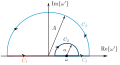
\includegraphics[width=8cm]{../../Figuras/integration.pdf}
		\caption{Parte imaginaria de la función dieléctrica. \textbf{a)} Función dieléctrica de eritrocitos con una concentración de 28.7 g/dL. Los datos experimentales se obtuvieron de \cite{friebelModelFunctionCalculate2006} y están indicados mediante puntos rojos. La línea azul continua representa el ajuste con lorentzianas obtenido. }
		\label{integration_contour}
	\end{figure}
	%
	
	\item Concentración 28.7 g/dL

	%
	\begin{figure}[h]
		\centering
		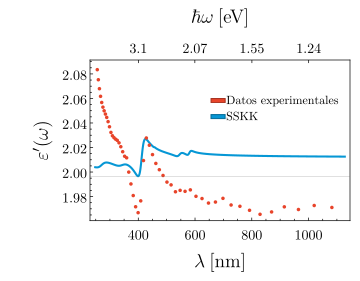
\includegraphics[width=8cm]{../../Figuras/sskk28.pdf}
		\caption{Parte imaginaria de la función dieléctrica. \textbf{a)} Función dieléctrica de eritrocitos con una concentración de 28.7 g/dL. Los datos experimentales se obtuvieron de \cite{friebelModelFunctionCalculate2006} y están indicados mediante puntos rojos. La línea azul continua representa el ajuste con lorentzianas obtenido. }
		\label{integration_contour}
	\end{figure}
	%
	
	
	\item Concentración 30.6 g/dL
	%
	\begin{figure}[h]
		\centering
		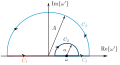
\includegraphics[width=8cm]{../../Figuras/integration.pdf}
		\caption{Parte imaginaria de la función dieléctrica. \textbf{a)} Función dieléctrica de eritrocitos con una concentración de 28.7 g/dL. Los datos experimentales se obtuvieron de \cite{friebelModelFunctionCalculate2006} y están indicados mediante puntos rojos. La línea azul continua representa el ajuste con lorentzianas obtenido. }
		\label{integration_contour}
	\end{figure}
	%
	
	
	
\end{itemize}